% Options for packages loaded elsewhere
\PassOptionsToPackage{unicode}{hyperref}
\PassOptionsToPackage{hyphens}{url}
%
\documentclass[
]{article}
\usepackage{amsmath,amssymb}
\usepackage{lmodern}
\usepackage{ifxetex,ifluatex}
\ifnum 0\ifxetex 1\fi\ifluatex 1\fi=0 % if pdftex
  \usepackage[T1]{fontenc}
  \usepackage[utf8]{inputenc}
  \usepackage{textcomp} % provide euro and other symbols
\else % if luatex or xetex
  \usepackage{unicode-math}
  \defaultfontfeatures{Scale=MatchLowercase}
  \defaultfontfeatures[\rmfamily]{Ligatures=TeX,Scale=1}
\fi
% Use upquote if available, for straight quotes in verbatim environments
\IfFileExists{upquote.sty}{\usepackage{upquote}}{}
\IfFileExists{microtype.sty}{% use microtype if available
  \usepackage[]{microtype}
  \UseMicrotypeSet[protrusion]{basicmath} % disable protrusion for tt fonts
}{}
\makeatletter
\@ifundefined{KOMAClassName}{% if non-KOMA class
  \IfFileExists{parskip.sty}{%
    \usepackage{parskip}
  }{% else
    \setlength{\parindent}{0pt}
    \setlength{\parskip}{6pt plus 2pt minus 1pt}}
}{% if KOMA class
  \KOMAoptions{parskip=half}}
\makeatother
\usepackage{xcolor}
\IfFileExists{xurl.sty}{\usepackage{xurl}}{} % add URL line breaks if available
\IfFileExists{bookmark.sty}{\usepackage{bookmark}}{\usepackage{hyperref}}
\hypersetup{
  pdftitle={Chosun Field},
  pdfauthor={coop711},
  hidelinks,
  pdfcreator={LaTeX via pandoc}}
\urlstyle{same} % disable monospaced font for URLs
\usepackage[margin=1in]{geometry}
\usepackage{color}
\usepackage{fancyvrb}
\newcommand{\VerbBar}{|}
\newcommand{\VERB}{\Verb[commandchars=\\\{\}]}
\DefineVerbatimEnvironment{Highlighting}{Verbatim}{commandchars=\\\{\}}
% Add ',fontsize=\small' for more characters per line
\usepackage{framed}
\definecolor{shadecolor}{RGB}{248,248,248}
\newenvironment{Shaded}{\begin{snugshade}}{\end{snugshade}}
\newcommand{\AlertTok}[1]{\textcolor[rgb]{0.94,0.16,0.16}{#1}}
\newcommand{\AnnotationTok}[1]{\textcolor[rgb]{0.56,0.35,0.01}{\textbf{\textit{#1}}}}
\newcommand{\AttributeTok}[1]{\textcolor[rgb]{0.77,0.63,0.00}{#1}}
\newcommand{\BaseNTok}[1]{\textcolor[rgb]{0.00,0.00,0.81}{#1}}
\newcommand{\BuiltInTok}[1]{#1}
\newcommand{\CharTok}[1]{\textcolor[rgb]{0.31,0.60,0.02}{#1}}
\newcommand{\CommentTok}[1]{\textcolor[rgb]{0.56,0.35,0.01}{\textit{#1}}}
\newcommand{\CommentVarTok}[1]{\textcolor[rgb]{0.56,0.35,0.01}{\textbf{\textit{#1}}}}
\newcommand{\ConstantTok}[1]{\textcolor[rgb]{0.00,0.00,0.00}{#1}}
\newcommand{\ControlFlowTok}[1]{\textcolor[rgb]{0.13,0.29,0.53}{\textbf{#1}}}
\newcommand{\DataTypeTok}[1]{\textcolor[rgb]{0.13,0.29,0.53}{#1}}
\newcommand{\DecValTok}[1]{\textcolor[rgb]{0.00,0.00,0.81}{#1}}
\newcommand{\DocumentationTok}[1]{\textcolor[rgb]{0.56,0.35,0.01}{\textbf{\textit{#1}}}}
\newcommand{\ErrorTok}[1]{\textcolor[rgb]{0.64,0.00,0.00}{\textbf{#1}}}
\newcommand{\ExtensionTok}[1]{#1}
\newcommand{\FloatTok}[1]{\textcolor[rgb]{0.00,0.00,0.81}{#1}}
\newcommand{\FunctionTok}[1]{\textcolor[rgb]{0.00,0.00,0.00}{#1}}
\newcommand{\ImportTok}[1]{#1}
\newcommand{\InformationTok}[1]{\textcolor[rgb]{0.56,0.35,0.01}{\textbf{\textit{#1}}}}
\newcommand{\KeywordTok}[1]{\textcolor[rgb]{0.13,0.29,0.53}{\textbf{#1}}}
\newcommand{\NormalTok}[1]{#1}
\newcommand{\OperatorTok}[1]{\textcolor[rgb]{0.81,0.36,0.00}{\textbf{#1}}}
\newcommand{\OtherTok}[1]{\textcolor[rgb]{0.56,0.35,0.01}{#1}}
\newcommand{\PreprocessorTok}[1]{\textcolor[rgb]{0.56,0.35,0.01}{\textit{#1}}}
\newcommand{\RegionMarkerTok}[1]{#1}
\newcommand{\SpecialCharTok}[1]{\textcolor[rgb]{0.00,0.00,0.00}{#1}}
\newcommand{\SpecialStringTok}[1]{\textcolor[rgb]{0.31,0.60,0.02}{#1}}
\newcommand{\StringTok}[1]{\textcolor[rgb]{0.31,0.60,0.02}{#1}}
\newcommand{\VariableTok}[1]{\textcolor[rgb]{0.00,0.00,0.00}{#1}}
\newcommand{\VerbatimStringTok}[1]{\textcolor[rgb]{0.31,0.60,0.02}{#1}}
\newcommand{\WarningTok}[1]{\textcolor[rgb]{0.56,0.35,0.01}{\textbf{\textit{#1}}}}
\usepackage{graphicx}
\makeatletter
\def\maxwidth{\ifdim\Gin@nat@width>\linewidth\linewidth\else\Gin@nat@width\fi}
\def\maxheight{\ifdim\Gin@nat@height>\textheight\textheight\else\Gin@nat@height\fi}
\makeatother
% Scale images if necessary, so that they will not overflow the page
% margins by default, and it is still possible to overwrite the defaults
% using explicit options in \includegraphics[width, height, ...]{}
\setkeys{Gin}{width=\maxwidth,height=\maxheight,keepaspectratio}
% Set default figure placement to htbp
\makeatletter
\def\fps@figure{htbp}
\makeatother
\setlength{\emergencystretch}{3em} % prevent overfull lines
\providecommand{\tightlist}{%
  \setlength{\itemsep}{0pt}\setlength{\parskip}{0pt}}
\setcounter{secnumdepth}{-\maxdimen} % remove section numbering
\ifluatex
  \usepackage{selnolig}  % disable illegal ligatures
\fi

\title{Chosun Field}
\author{coop711}
\date{}

\begin{document}
\maketitle

\hypertarget{problem}{%
\subsection{Problem}\label{problem}}

조선시대 전답 통계를 stacked area graph로 표시

\begin{Shaded}
\begin{Highlighting}[]
\FunctionTok{options}\NormalTok{(}\AttributeTok{warn =} \SpecialCharTok{{-}}\DecValTok{1}\NormalTok{)}
\FunctionTok{library}\NormalTok{(knitr)}
\FunctionTok{library}\NormalTok{(magrittr)}
\FunctionTok{library}\NormalTok{(showtext)}
\end{Highlighting}
\end{Shaded}

\begin{verbatim}
## Loading required package: sysfonts
\end{verbatim}

\begin{verbatim}
## Loading required package: showtextdb
\end{verbatim}

\begin{Shaded}
\begin{Highlighting}[]
\FunctionTok{include\_graphics}\NormalTok{(}\StringTok{"../pics/chosun\_field\_history.png"}\NormalTok{)}
\end{Highlighting}
\end{Shaded}

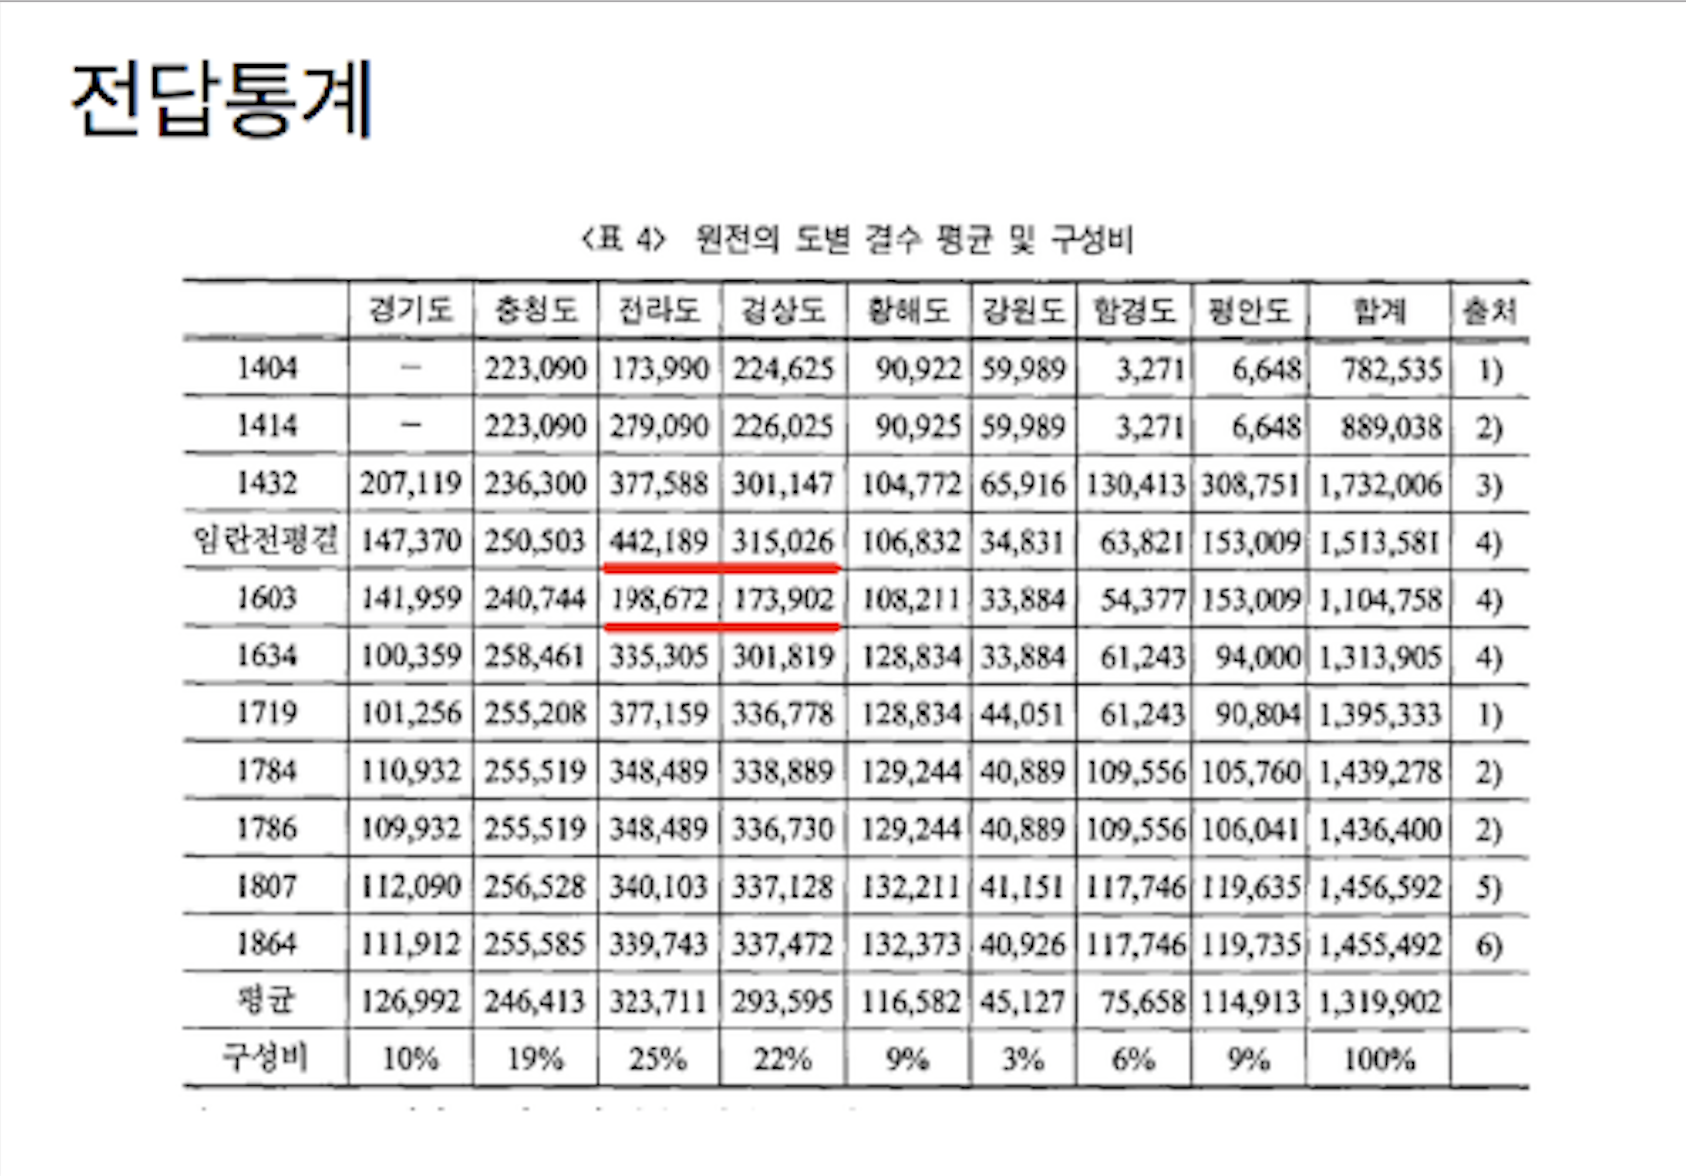
\includegraphics[width=0.8\linewidth]{../pics/chosun_field_history}

\hypertarget{data}{%
\subsection{Data}\label{data}}

\begin{Shaded}
\begin{Highlighting}[]
\FunctionTok{library}\NormalTok{(knitr)}
\NormalTok{Year }\OtherTok{\textless{}{-}} \FunctionTok{c}\NormalTok{(}\DecValTok{1404}\NormalTok{, }\DecValTok{1414}\NormalTok{, }\DecValTok{1432}\NormalTok{, }\DecValTok{1592}\NormalTok{, }\DecValTok{1603}\NormalTok{, }\DecValTok{1634}\NormalTok{, }\DecValTok{1719}\NormalTok{, }\DecValTok{1784}\NormalTok{, }\DecValTok{1786}\NormalTok{, }\DecValTok{1807}\NormalTok{, }\DecValTok{1864}\NormalTok{)}
\NormalTok{Province }\OtherTok{\textless{}{-}} \FunctionTok{c}\NormalTok{(}\StringTok{"경기도"}\NormalTok{, }\StringTok{"충청도"}\NormalTok{, }\StringTok{"전라도"}\NormalTok{, }\StringTok{"경상도"}\NormalTok{, }\StringTok{"황해도"}\NormalTok{, }\StringTok{"강원도"}\NormalTok{, }\StringTok{"함경도"}\NormalTok{, }\StringTok{"평안도"}\NormalTok{)}
\NormalTok{field }\OtherTok{\textless{}{-}} \FunctionTok{matrix}\NormalTok{(}\FunctionTok{c}\NormalTok{(}\ConstantTok{NA}\NormalTok{, }\DecValTok{223090}\NormalTok{, }\DecValTok{173990}\NormalTok{, }\DecValTok{224625}\NormalTok{, }\DecValTok{90922}\NormalTok{, }\DecValTok{59989}\NormalTok{, }\DecValTok{3271}\NormalTok{, }\DecValTok{6648}\NormalTok{,}
                  \ConstantTok{NA}\NormalTok{, }\DecValTok{223090}\NormalTok{, }\DecValTok{279090}\NormalTok{, }\DecValTok{226025}\NormalTok{, }\DecValTok{90925}\NormalTok{, }\DecValTok{59989}\NormalTok{, }\DecValTok{3271}\NormalTok{, }\DecValTok{6648}\NormalTok{,}
                  \DecValTok{207119}\NormalTok{, }\DecValTok{236300}\NormalTok{, }\DecValTok{377588}\NormalTok{, }\DecValTok{301147}\NormalTok{, }\DecValTok{104772}\NormalTok{, }\DecValTok{65916}\NormalTok{, }\DecValTok{130413}\NormalTok{, }\DecValTok{308751}\NormalTok{, }
                  \DecValTok{147370}\NormalTok{, }\DecValTok{250503}\NormalTok{, }\DecValTok{442189}\NormalTok{, }\DecValTok{315026}\NormalTok{, }\DecValTok{106832}\NormalTok{, }\DecValTok{34831}\NormalTok{, }\DecValTok{63821}\NormalTok{, }\DecValTok{153009}\NormalTok{,}
                  \DecValTok{141959}\NormalTok{, }\DecValTok{240744}\NormalTok{, }\DecValTok{198672}\NormalTok{, }\DecValTok{173902}\NormalTok{, }\DecValTok{108211}\NormalTok{, }\DecValTok{33884}\NormalTok{, }\DecValTok{54377}\NormalTok{, }\DecValTok{153009}\NormalTok{,}
                  \DecValTok{100359}\NormalTok{, }\DecValTok{258461}\NormalTok{, }\DecValTok{335305}\NormalTok{, }\DecValTok{301819}\NormalTok{, }\DecValTok{128834}\NormalTok{, }\DecValTok{33884}\NormalTok{, }\DecValTok{61243}\NormalTok{, }\DecValTok{94000}\NormalTok{,}
                  \DecValTok{101256}\NormalTok{, }\DecValTok{255208}\NormalTok{, }\DecValTok{377159}\NormalTok{, }\DecValTok{336778}\NormalTok{, }\DecValTok{128834}\NormalTok{, }\DecValTok{44051}\NormalTok{, }\DecValTok{61243}\NormalTok{, }\DecValTok{90804}\NormalTok{,}
                  \DecValTok{110932}\NormalTok{, }\DecValTok{255519}\NormalTok{, }\DecValTok{348489}\NormalTok{, }\DecValTok{335730}\NormalTok{, }\DecValTok{129244}\NormalTok{, }\DecValTok{40889}\NormalTok{, }\DecValTok{109556}\NormalTok{, }\DecValTok{105760}\NormalTok{,}
                  \DecValTok{109932}\NormalTok{, }\DecValTok{255519}\NormalTok{, }\DecValTok{348489}\NormalTok{, }\DecValTok{336730}\NormalTok{, }\DecValTok{129244}\NormalTok{, }\DecValTok{40889}\NormalTok{, }\DecValTok{109556}\NormalTok{, }\DecValTok{106041}\NormalTok{,}
                  \DecValTok{112090}\NormalTok{, }\DecValTok{256528}\NormalTok{, }\DecValTok{340103}\NormalTok{, }\DecValTok{337128}\NormalTok{, }\DecValTok{132211}\NormalTok{, }\DecValTok{41151}\NormalTok{, }\DecValTok{117746}\NormalTok{, }\DecValTok{119635}\NormalTok{, }
                  \DecValTok{111912}\NormalTok{, }\DecValTok{255585}\NormalTok{, }\DecValTok{339743}\NormalTok{, }\DecValTok{337472}\NormalTok{, }\DecValTok{132373}\NormalTok{, }\DecValTok{40926}\NormalTok{, }\DecValTok{117746}\NormalTok{, }\DecValTok{119735}\NormalTok{), }
                \AttributeTok{ncol =} \DecValTok{8}\NormalTok{, }
                \AttributeTok{byrow =} \ConstantTok{TRUE}\NormalTok{)}
\FunctionTok{rownames}\NormalTok{(field) }\OtherTok{\textless{}{-}}\NormalTok{ Year}
\FunctionTok{colnames}\NormalTok{(field) }\OtherTok{\textless{}{-}}\NormalTok{ Province}
\NormalTok{field }\SpecialCharTok{\%\textgreater{}\%}\NormalTok{ str}
\end{Highlighting}
\end{Shaded}

\begin{verbatim}
##  num [1:11, 1:8] NA NA 207119 147370 141959 ...
##  - attr(*, "dimnames")=List of 2
##   ..$ : chr [1:11] "1404" "1414" "1432" "1592" ...
##   ..$ : chr [1:8] "경기도" "충청도" "전라도" "경상도" ...
\end{verbatim}

\begin{Shaded}
\begin{Highlighting}[]
\FunctionTok{options}\NormalTok{(}\AttributeTok{digits =} \DecValTok{2}\NormalTok{)}
\NormalTok{mean\_field }\OtherTok{\textless{}{-}}\NormalTok{ field }\SpecialCharTok{\%\textgreater{}\%} \FunctionTok{colMeans}\NormalTok{(}\AttributeTok{na.rm =} \ConstantTok{TRUE}\NormalTok{)}
\NormalTok{prop\_field }\OtherTok{\textless{}{-}}\NormalTok{ field }\SpecialCharTok{\%\textgreater{}\%} 
\NormalTok{  \{}\FunctionTok{colMeans}\NormalTok{(., }\AttributeTok{na.rm =} \ConstantTok{TRUE}\NormalTok{) }\SpecialCharTok{/} \FunctionTok{sum}\NormalTok{(}\FunctionTok{colMeans}\NormalTok{(., }\AttributeTok{na.rm =} \ConstantTok{TRUE}\NormalTok{))\} }\SpecialCharTok{\%\textgreater{}\%}
  \StringTok{\textasciigrave{}}\AttributeTok{*}\StringTok{\textasciigrave{}}\NormalTok{(}\DecValTok{100}\NormalTok{) }\SpecialCharTok{\%\textgreater{}\%}
  \FunctionTok{round}\NormalTok{(}\AttributeTok{digits =} \DecValTok{2}\NormalTok{)}
\end{Highlighting}
\end{Shaded}

\hypertarget{reshape}{%
\subsection{Reshape}\label{reshape}}

\texttt{matrix} (array)에 특화된 \texttt{melt} 사용

\begin{Shaded}
\begin{Highlighting}[]
\FunctionTok{library}\NormalTok{(reshape2)}
\NormalTok{field\_melt }\OtherTok{\textless{}{-}}\NormalTok{ field }\SpecialCharTok{\%\textgreater{}\%}
  \FunctionTok{melt}\NormalTok{(}\AttributeTok{varnames =} \FunctionTok{c}\NormalTok{(}\StringTok{"Year"}\NormalTok{, }\StringTok{"Province"}\NormalTok{), }\AttributeTok{value.name =} \StringTok{"Area"}\NormalTok{)}
\NormalTok{field\_melt }\SpecialCharTok{\%\textgreater{}\%}\NormalTok{ str}
\end{Highlighting}
\end{Shaded}

\begin{verbatim}
## 'data.frame':    88 obs. of  3 variables:
##  $ Year    : int  1404 1414 1432 1592 1603 1634 1719 1784 1786 1807 ...
##  $ Province: Factor w/ 8 levels "경기도","충청도",..: 1 1 1 1 1 1 1 1 1 1 ...
##  $ Area    : num  NA NA 207119 147370 141959 ...
\end{verbatim}

\begin{Shaded}
\begin{Highlighting}[]
\CommentTok{\# kable(field\_melt)}
\end{Highlighting}
\end{Shaded}

\hypertarget{ggplot}{%
\subsection{ggplot}\label{ggplot}}

\begin{Shaded}
\begin{Highlighting}[]
\FunctionTok{library}\NormalTok{(ggplot2)}
\FunctionTok{library}\NormalTok{(extrafont)}
\FunctionTok{showtext\_auto}\NormalTok{()}
\FunctionTok{font\_add}\NormalTok{(}\AttributeTok{family =} \StringTok{"KoPubWorld Dotum Medium"}\NormalTok{, }\AttributeTok{regular =} \StringTok{"KoPubWorld/KoPubWorld Dotum Medium.ttf"}\NormalTok{)}
\FunctionTok{font\_add}\NormalTok{(}\AttributeTok{family =} \StringTok{"KoPubWorld Dotum Bold"}\NormalTok{, }\AttributeTok{regular =} \StringTok{"KoPubWorld/KoPubWorld Dotum Bold.ttf"}\NormalTok{)}
\NormalTok{g0 }\OtherTok{\textless{}{-}} \FunctionTok{ggplot}\NormalTok{()}
\NormalTok{g1 }\OtherTok{\textless{}{-}}\NormalTok{ g0 }\SpecialCharTok{+}
  \FunctionTok{geom\_area}\NormalTok{(}\AttributeTok{data =}\NormalTok{ field\_melt, }
            \AttributeTok{mapping =} \FunctionTok{aes}\NormalTok{(}\AttributeTok{x =}\NormalTok{ Year, }\AttributeTok{y =}\NormalTok{ Area, }\AttributeTok{fill =}\NormalTok{ Province),}
            \AttributeTok{colour =} \StringTok{"black"}\NormalTok{, }
            \AttributeTok{size =} \FloatTok{0.2}\NormalTok{, }
            \AttributeTok{alpha =} \FloatTok{0.4}\NormalTok{, }
            \AttributeTok{na.rm =} \ConstantTok{TRUE}\NormalTok{)}
\NormalTok{g1}
\end{Highlighting}
\end{Shaded}

\includegraphics{Chosun_Field_p_files/figure-latex/ggplot-1.pdf}

\begin{Shaded}
\begin{Highlighting}[]
\NormalTok{g2 }\OtherTok{\textless{}{-}}\NormalTok{ g1 }\SpecialCharTok{+}
  \FunctionTok{scale\_fill\_brewer}\NormalTok{(}\AttributeTok{palette =} \StringTok{"Spectral"}\NormalTok{, }
                    \AttributeTok{name =} \StringTok{""}\NormalTok{,}
                    \AttributeTok{breaks =} \FunctionTok{levels}\NormalTok{(field\_melt}\SpecialCharTok{$}\NormalTok{Province)) }\SpecialCharTok{+}
  \FunctionTok{theme\_bw}\NormalTok{()}
\NormalTok{g2}
\end{Highlighting}
\end{Shaded}

\includegraphics{Chosun_Field_p_files/figure-latex/ggplot2-1.pdf}

\begin{Shaded}
\begin{Highlighting}[]
\NormalTok{g3}\OtherTok{\textless{}{-}}\NormalTok{ g2 }\SpecialCharTok{+} 
  \FunctionTok{scale\_x\_continuous}\NormalTok{(}\AttributeTok{name =} \StringTok{"연도"}\NormalTok{, }
                     \AttributeTok{breaks =} \FunctionTok{as.numeric}\NormalTok{(}\FunctionTok{row.names}\NormalTok{(field)[}\SpecialCharTok{{-}}\DecValTok{9}\NormalTok{]),}
                     \AttributeTok{labels =} \FunctionTok{row.names}\NormalTok{(field)[}\SpecialCharTok{{-}}\DecValTok{9}\NormalTok{])}
\NormalTok{g3}
\end{Highlighting}
\end{Shaded}

\includegraphics{Chosun_Field_p_files/figure-latex/unnamed-chunk-2-1.pdf}

\begin{Shaded}
\begin{Highlighting}[]
\NormalTok{g4 }\OtherTok{\textless{}{-}}\NormalTok{ g3 }\SpecialCharTok{+}
  \FunctionTok{theme}\NormalTok{(}\AttributeTok{axis.text.x =} \FunctionTok{element\_text}\NormalTok{(}\AttributeTok{angle =} \DecValTok{90}\NormalTok{))}
\NormalTok{g4}
\end{Highlighting}
\end{Shaded}

\includegraphics{Chosun_Field_p_files/figure-latex/unnamed-chunk-3-1.pdf}

\begin{Shaded}
\begin{Highlighting}[]
\NormalTok{g5 }\OtherTok{\textless{}{-}}\NormalTok{ g4 }\SpecialCharTok{+} 
  \FunctionTok{scale\_y\_continuous}\NormalTok{(}\AttributeTok{name =} \StringTok{"토지 면적(결)"}\NormalTok{,}
                     \AttributeTok{breaks =} \FunctionTok{cumsum}\NormalTok{(}\FunctionTok{rev}\NormalTok{(field[}\DecValTok{3}\NormalTok{, ])),}
                     \AttributeTok{labels =} \FunctionTok{format}\NormalTok{(}\FunctionTok{cumsum}\NormalTok{(}\FunctionTok{rev}\NormalTok{(field[}\DecValTok{3}\NormalTok{, ])), }\AttributeTok{big.mark =} \StringTok{","}\NormalTok{))}
\NormalTok{g5}
\end{Highlighting}
\end{Shaded}

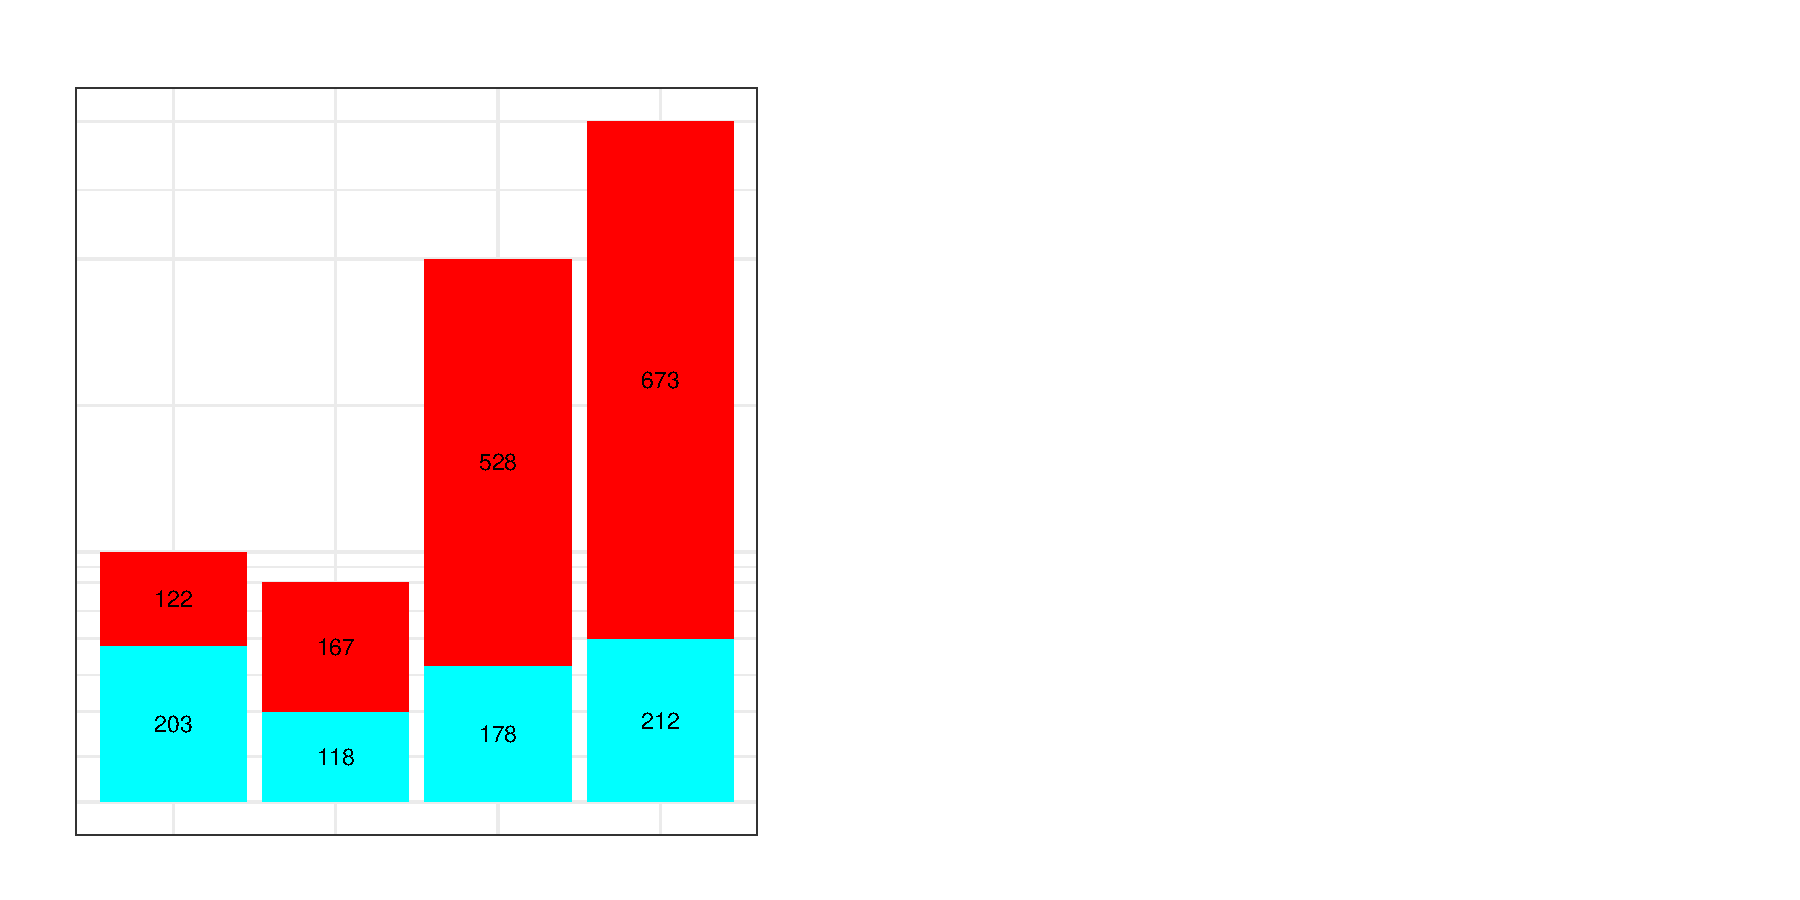
\includegraphics{Chosun_Field_p_files/figure-latex/unnamed-chunk-4-1.pdf}

\begin{Shaded}
\begin{Highlighting}[]
\NormalTok{g6 }\OtherTok{\textless{}{-}}\NormalTok{ g5 }\SpecialCharTok{+}
  \FunctionTok{labs}\NormalTok{(}\AttributeTok{title =} \StringTok{"조선 시대 도별 논밭통계"}\NormalTok{, }
       \AttributeTok{subtitle =} \StringTok{"(도표 안의 수치는 기록된 값들의 평균)"}\NormalTok{) }\SpecialCharTok{+}
  \FunctionTok{theme}\NormalTok{(}\AttributeTok{plot.subtitle =} \FunctionTok{element\_text}\NormalTok{(}\AttributeTok{family =} \StringTok{"KoPubWorldDotum Medium"}\NormalTok{, }
                                     \AttributeTok{hjust =} \DecValTok{1}\NormalTok{))}
\NormalTok{g6}
\end{Highlighting}
\end{Shaded}

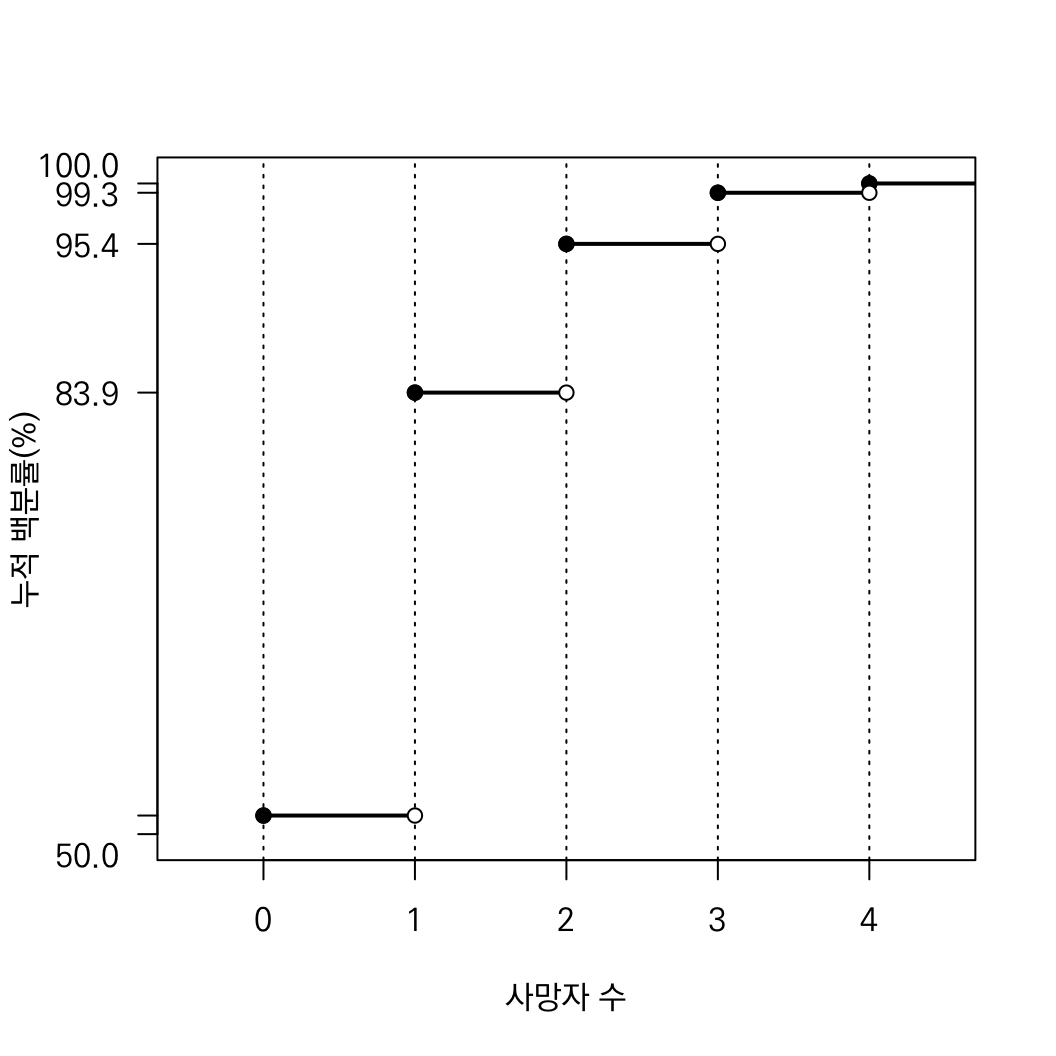
\includegraphics{Chosun_Field_p_files/figure-latex/unnamed-chunk-5-1.pdf}

\begin{Shaded}
\begin{Highlighting}[]
\NormalTok{g7 }\OtherTok{\textless{}{-}}\NormalTok{ g6 }\SpecialCharTok{+}
  \FunctionTok{theme}\NormalTok{(}\AttributeTok{plot.title =} \FunctionTok{element\_text}\NormalTok{(}\AttributeTok{size =} \DecValTok{20}\NormalTok{, }
                                  \AttributeTok{hjust =} \FloatTok{0.5}\NormalTok{,}
                                  \AttributeTok{family =} \StringTok{"KoPubWorldDotum Bold"}\NormalTok{))}
\NormalTok{g7}
\end{Highlighting}
\end{Shaded}

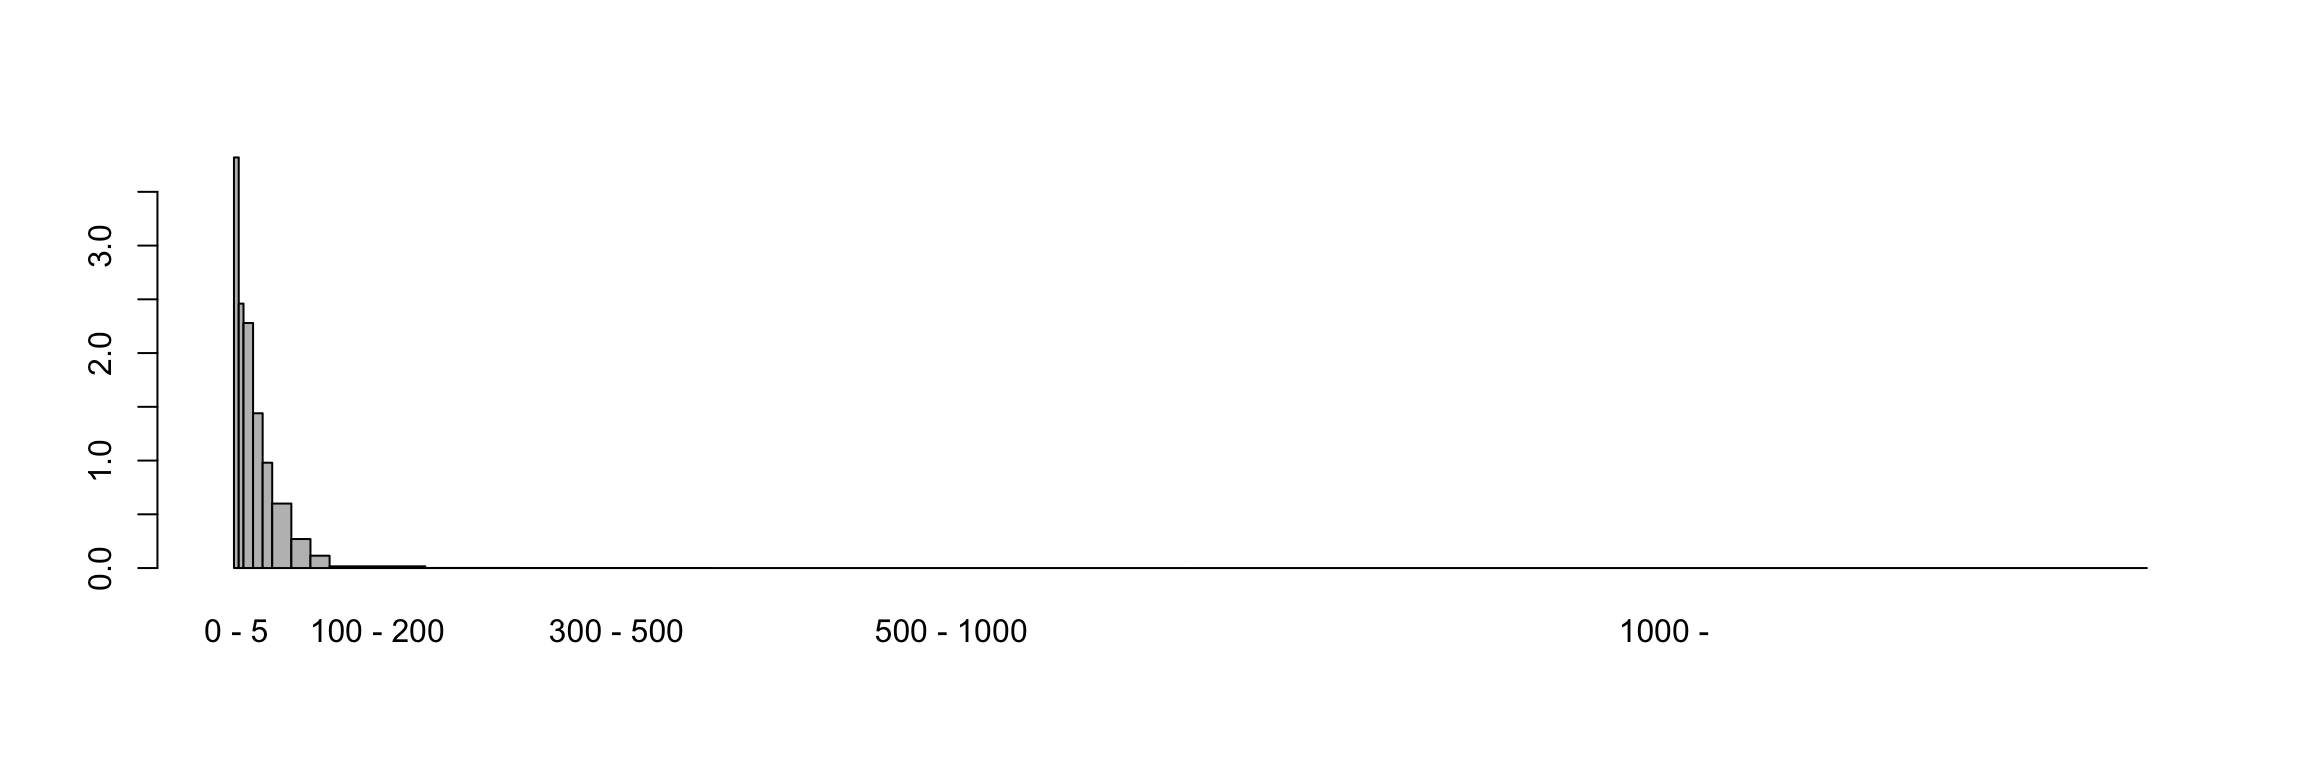
\includegraphics{Chosun_Field_p_files/figure-latex/unnamed-chunk-6-1.pdf}

\begin{Shaded}
\begin{Highlighting}[]
\CommentTok{\#  x.max \textless{}{-} max(Year) + 0.15 * diff(range(Year))}
\CommentTok{\# g8 \textless{}{-} g7 +}
\CommentTok{\#  scale\_x\_continuous(name = "연도", }
\CommentTok{\#                     breaks = as.numeric(row.names(field)[{-}9]),}
\CommentTok{\#                     labels = row.names(field)[{-}9],}
\CommentTok{\#                     limits = c(min(Year), x.max)) +}
\CommentTok{\#  theme(legend.position = c(0.95, 0.5),}
\CommentTok{\#        legend.box.background = element\_rect(fill = "white", colour = "black"),}
\CommentTok{\#        legend.title = element\_blank())}
\CommentTok{\# g8}
\NormalTok{g9 }\OtherTok{\textless{}{-}}\NormalTok{ g7 }\SpecialCharTok{+}
  \FunctionTok{theme}\NormalTok{(}\AttributeTok{legend.position =} \FunctionTok{c}\NormalTok{(}\FloatTok{0.75}\NormalTok{, }\FloatTok{0.9}\NormalTok{),}
        \AttributeTok{legend.box.background =} \FunctionTok{element\_rect}\NormalTok{(}\AttributeTok{fill =} \StringTok{"white"}\NormalTok{, }\AttributeTok{colour =} \StringTok{"black"}\NormalTok{),}
        \AttributeTok{legend.direction =} \StringTok{"horizontal"}\NormalTok{)}
\NormalTok{g9}
\end{Highlighting}
\end{Shaded}

\includegraphics{Chosun_Field_p_files/figure-latex/unnamed-chunk-7-1.pdf}

\begin{Shaded}
\begin{Highlighting}[]
\NormalTok{y\_coord }\OtherTok{\textless{}{-}} \FunctionTok{apply}\NormalTok{(field[}\DecValTok{3}\SpecialCharTok{:}\DecValTok{4}\NormalTok{, ], }\DecValTok{2}\NormalTok{, mean)}
\NormalTok{y\_text }\OtherTok{\textless{}{-}} \FunctionTok{cumsum}\NormalTok{(}\FunctionTok{c}\NormalTok{(}\DecValTok{0}\NormalTok{, }\FunctionTok{head}\NormalTok{(}\FunctionTok{rev}\NormalTok{(y\_coord), }\SpecialCharTok{{-}}\DecValTok{1}\NormalTok{))) }\SpecialCharTok{+} \FunctionTok{rev}\NormalTok{(y\_coord) }\SpecialCharTok{/} \DecValTok{2}
\NormalTok{mean\_text }\OtherTok{\textless{}{-}} \FunctionTok{rev}\NormalTok{(}\FunctionTok{paste}\NormalTok{(Province, }
                       \StringTok{":"}\NormalTok{, }
                       \FunctionTok{format}\NormalTok{(mean\_field, }\AttributeTok{big.mark =} \StringTok{","}\NormalTok{), }
                       \StringTok{"결("}\NormalTok{, }
                       \FunctionTok{format}\NormalTok{(prop\_field, }\AttributeTok{digits =} \DecValTok{2}\NormalTok{, }\AttributeTok{nsmall =} \DecValTok{0}\NormalTok{), }
                       \StringTok{"\%)"}\NormalTok{, }
                       \AttributeTok{sep =} \StringTok{""}\NormalTok{))}
\NormalTok{text\_df }\OtherTok{\textless{}{-}} \FunctionTok{data.frame}\NormalTok{(}\AttributeTok{x =}\NormalTok{ (Year[}\DecValTok{3}\NormalTok{] }\SpecialCharTok{+}\NormalTok{ Year[}\DecValTok{4}\NormalTok{]) }\SpecialCharTok{/} \DecValTok{2}\NormalTok{, }
                      \AttributeTok{y =}\NormalTok{ y\_text, }
                      \AttributeTok{label =}\NormalTok{ mean\_text, }
                      \AttributeTok{row.names =} \ConstantTok{NULL}\NormalTok{, }
                      \AttributeTok{stringsAsFactors =} \ConstantTok{FALSE}\NormalTok{)}
\end{Highlighting}
\end{Shaded}

\begin{Shaded}
\begin{Highlighting}[]
\NormalTok{g10 }\OtherTok{\textless{}{-}}\NormalTok{ g9 }\SpecialCharTok{+}
  \FunctionTok{guides}\NormalTok{(}\AttributeTok{fill =} \ConstantTok{FALSE}\NormalTok{) }\SpecialCharTok{+}
  \FunctionTok{geom\_text}\NormalTok{(}\AttributeTok{data =}\NormalTok{ text\_df, }
            \AttributeTok{mapping =} \FunctionTok{aes}\NormalTok{(}\AttributeTok{x =}\NormalTok{ x, }\AttributeTok{y =}\NormalTok{ y), }
            \AttributeTok{label =}\NormalTok{ mean\_text, }
            \AttributeTok{family =} \StringTok{"KoPubWorldDotum Medium"}\NormalTok{, }\AttributeTok{size =} \DecValTok{3}\NormalTok{) }\SpecialCharTok{+}
  \FunctionTok{annotate}\NormalTok{(}\StringTok{"text"}\NormalTok{, }\AttributeTok{x =} \DecValTok{1592}\NormalTok{, }\AttributeTok{y =} \DecValTok{1650000}\NormalTok{, }
           \AttributeTok{label =} \StringTok{"임진왜란"}\NormalTok{, }
           \AttributeTok{colour =} \StringTok{"red"}\NormalTok{,}
           \AttributeTok{size =} \DecValTok{5}\NormalTok{,}
           \AttributeTok{family =} \StringTok{"KoPubWorldDotum Medium"}\NormalTok{)}
\CommentTok{\#  theme(text = element\_text(family = "KoPubWorldDotum Medium"))}
\CommentTok{\#  annotate("text", }
\CommentTok{\#           x = text\_df$x, }
\CommentTok{\#           y = text\_df$y, }
\CommentTok{\#           label = mean\_text, }
\CommentTok{\#           family = "KoPubWorldDotum Medium")}

\NormalTok{g10}
\end{Highlighting}
\end{Shaded}

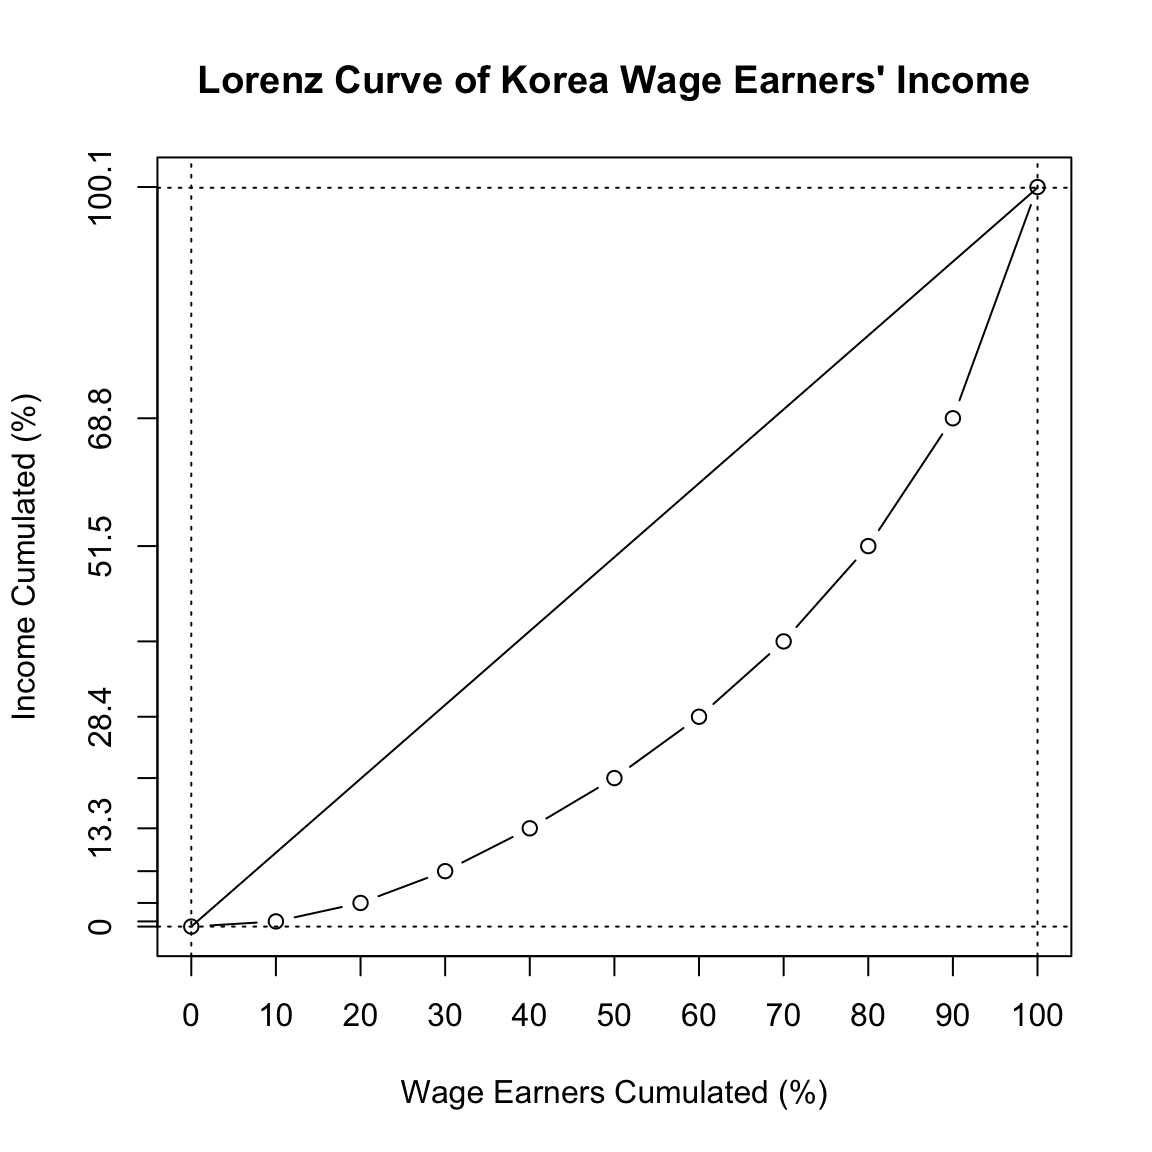
\includegraphics{Chosun_Field_p_files/figure-latex/unnamed-chunk-9-1.pdf}

\begin{Shaded}
\begin{Highlighting}[]
\FunctionTok{ggsave}\NormalTok{(}\StringTok{"../pics/chosun\_field\_ggplot.png"}\NormalTok{, }\AttributeTok{dpi =} \DecValTok{72}\NormalTok{)}
\end{Highlighting}
\end{Shaded}


\end{document}
